\newpage

\section{Partie 1: Quelques opérations de base sur les signaux}

\subsection{Signal numérique de synthèse}

\subsubsection{Génération du signal}

Un signal sinusoïdal de fréquence \( f_0 \) est généré par la fonction suivante:

\[
x[n] = \sin\left(2\pi f_0 \frac{n}{f_e}\right)
\]

où \( f_e \) est la fréquence d’échantillonnage et \( N \) le nombre d’échantillons.

\begin{figure}[!h]
\centering
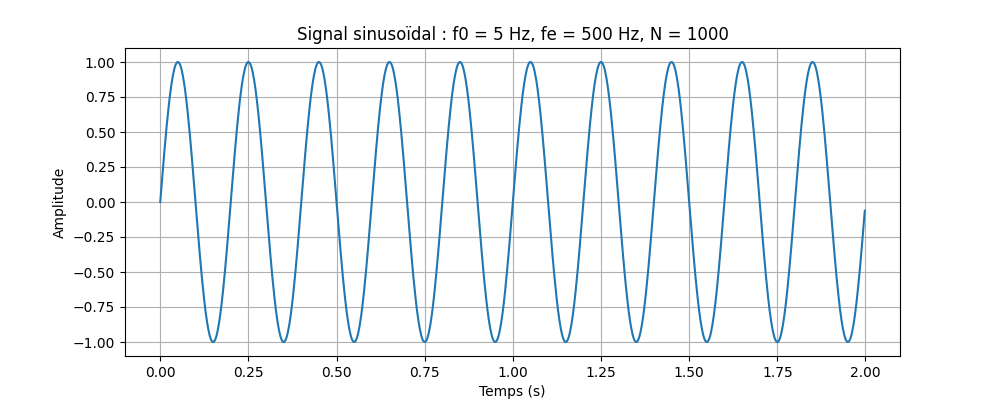
\includegraphics[width=17cm]{screenshots/signal_echantillone.png}
\caption{Signal sinusoïdal échantillonné}
\end{figure}

\subsubsection{Énergie et puissance}

L'énergie d’un signal discret \( x[n] \) est donnée par :

\[
E = \sum_{n=0}^{N-1} x[n]^2
\]

Et la puissance moyenne par :

\[
P = \frac{1}{N} \sum_{n=0}^{N-1} x[n]^2
\]

Considérons un signal sinusoïdal discret de la forme :
\[
x[n] = A \cdot \sin\left(2\pi f_0 \frac{n}{f_e} \right)
\]

La puissance moyenne théorique d’un signal périodique est calculée par la  formule:

\[
P = \lim_{N \to \infty} \frac{1}{N} \sum_{n=0}^{N-1} x[n]^2
\]

En utilisant l’identité trigonométrique :
\[
\sin^2(\theta) = \frac{1 - \cos(2\theta)}{2}
\]
on obtient :
\[
x[n]^2 = A^2 \cdot \frac{1 - \cos\left(4\pi f_0 \frac{n}{f_e} \right)}{2}
\]

Ainsi, la puissance devient :
\[
P = \lim_{N \to \infty} \frac{1}{N} \sum_{n=0}^{N-1} A^2 \cdot \frac{1 - \cos\left(4\pi f_0 \frac{n}{f_e} \right)}{2}
= \lim_{N \to \infty}  \frac{A^2}{2} - \frac{A^2}{2N} \sum_{n=0}^{N-1} \cos\left(4\pi f_0 \frac{n}{f_e} \right)
= \frac{A^2}{2}
\] 

Donc dans notre cas la puissance moyenne théorique est égale à 0.5.

Pour la puissance moyenne calculée numériquement pour le signal échantillonné on a la méme formule mais sans la limite:

\[
P = \frac{A^2}{2} - \frac{A^2}{2N} \sum_{n=0}^{N-1} \cos\left(4\pi f_0 \frac{n}{f_e} \right)
\] 

\textbf{Cas idéal :} si $N$ est un multiple entier de la période du signal (i.e., $N$ couvre un nombre entier de périodes), alors la somme des cosinus s’annule :
\[
\sum_{n=0}^{N-1} \cos\left(4\pi f_0 t \right) = 0 \quad \Rightarrow \quad P = \frac{A^2}{2}
\]

\textbf{Cas général :} si $N$ n’est pas un multiple exact de la période, la somme ne s’annule pas et on observe une légère déviation de la puissance par rapport à $\frac{A^2}{2}$. Cela est dû au fait que le signal est tronqué entre deux points non symétriques.\\

En variant N on trouve plusieurs valeurs de la puissance moyenne qui restent proches de la valeur théorique:

\begin{figure}[!h]
\centering
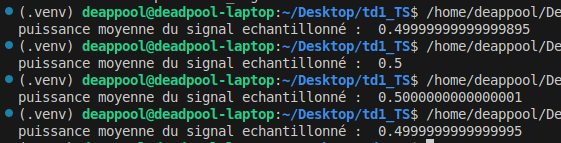
\includegraphics[width=15cm]{screenshots/puissance_et_energie.png}
\caption{Énergie et puissance du signal}
\end{figure}

\subsubsection{Quantification}

\begin{figure}[!h]
\centering
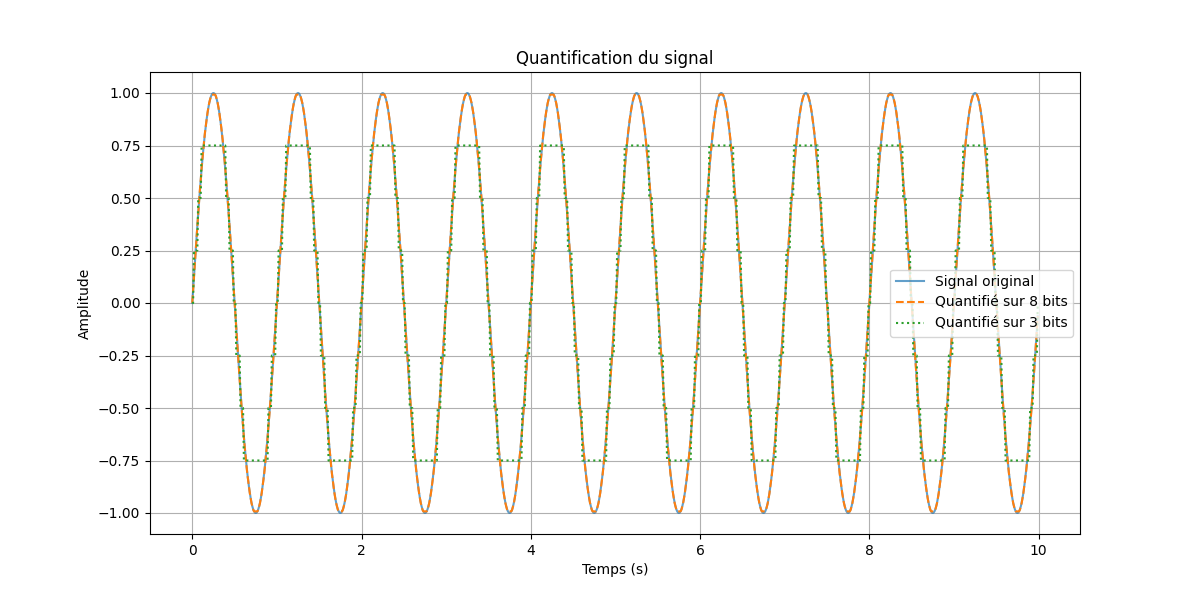
\includegraphics[width=15.5cm]{screenshots/quantification_graph.png}
\caption{Quantification du signal à 3 et 8 bits}
\end{figure}

Pour la quantification à 3 bits, on retrouve bien 8 niveaux de quantification.

\begin{figure}[!h]
\centering
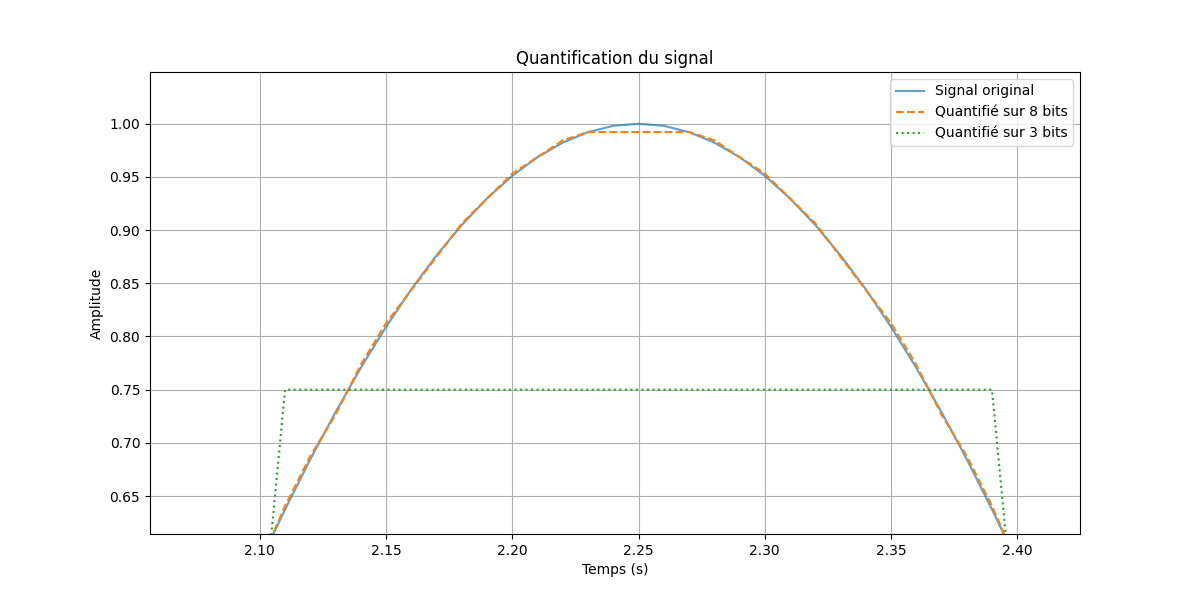
\includegraphics[width=17cm]{screenshots/quantification_graph_zoomed.png}
\caption{Zoom sur la quantification du signal à 3 et 8 bits}
\end{figure}

Le signal à 8 bits suit mieux la forme continue du signal d’origine mais on voit quand méme quelques erruers. À 3 bits, les marches sont plus visibles et le signal produit est significativement moins fidéle au signal d'origine.\\

\textbf{SNR (Signal-to-Noise Ratio)} :

\[
\text{SNR} = 10 \log_{10} \left(\frac{E_{\text{signal}}}{E_{\text{bruit}}} \right)
\]

\begin{figure}[!h]
\centering
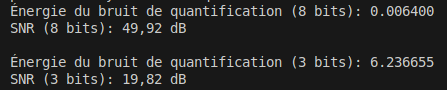
\includegraphics{screenshots/snr_quantification.png}
\caption{SNR pour chaque niveau de quantification}
\end{figure}

On remarque que l'energie du bruit est plus élevée pour le signal quantifié à 3 bits. Le résultat est logique
car on voit sur le graphe que ce signal est plus éloigné du signal d'origine comparé au signal quantifié à 8 bits.
On a la méme conclusion en raisonant sur le SNR: SNRq8 > SNRq3.

\subsection{Signal audio}

\subsubsection{Enregistrement}

Les mots « Bonjour » et « ChatGpt » ont été enregistrés via Audacity (voir figure \ref{fig:signal_enregistre}).

\subsubsection{Restitution à différentes fréquences}

L’audio est lu à \( f_e \), \( 2 f_e \) et \( \frac{f_e}{2} \). 

\textbf{Effets observés} :

\begin{itemize}
    \item \textbf{Durée :} doubler la fréquence de restitution divise la durée par deux (voix accélérée), tandis que la diviser par deux double la durée (voix ralentie).
    \item \textbf{Hauteur :} multiplier la fréquence de restitution rend la voix plus aiguë (fréquences doublées), la diminuer la rend plus grave (fréquences divisées).
\end{itemize}

Lorsque la fréquence de restitution est trop grande ou trop petite comparée à la fréquence d’échantillonnage, le son devient incompréhensible. Le son est trop rapide ou trop lent, mais aussi on ne reconnaît plus les mots. Cela s'explique notamment par le déplacement des formants, c’est-à-dire des pics de résonance caractéristiques des voyelles et consonnes, qui changent de position dans le spectre. Leur modification rend la parole méconnaissable, car ce sont eux qui permettent d’identifier les sons du langage.

\subsubsection{Quantification du signal audio}

\begin{itemize}
    \item À 3 bits : le son devient rugueux et très bruité, fortement altéré.
    \item À 8 bits : la voix reste compréhensible mais moins naturelle.
\end{itemize}

\subsubsection{Extraction et séparation de mots}

Après repérage visuel, les deux mots ont été extraits via tranches temporelles.


\begin{figure}[!h]
\centering
\includegraphics[width=10cm]{screenshots/signal_enregistré.png}
\caption{Signal audio enregistré}
\label{fig:signal_enregistre}
\end{figure}

\begin{figure}[h]
\centering
\begin{subfigure}[b]{0.45\textwidth}
    \centering
    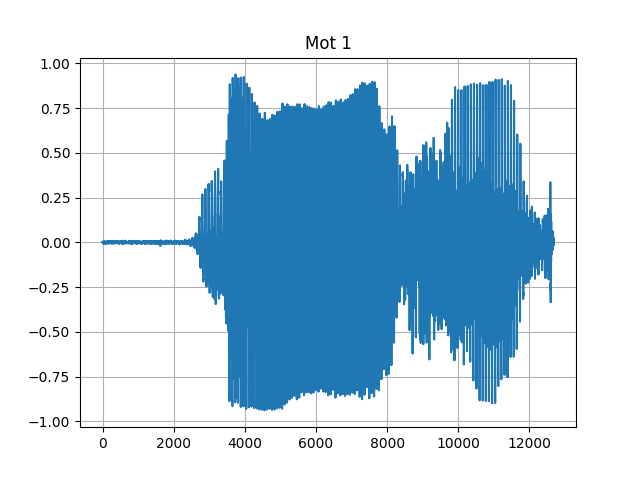
\includegraphics[width=9cm]{screenshots/mot1_graphe.png}
    \caption{Mot 1: "Bonjour"}
\end{subfigure}
\hfill
\begin{subfigure}[b]{0.45\textwidth}
    \centering
    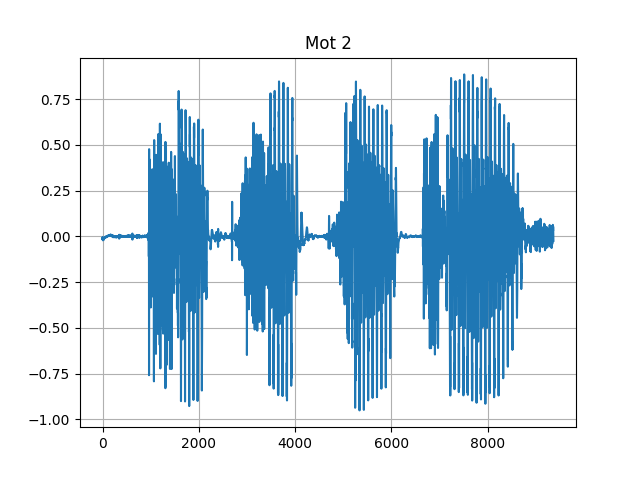
\includegraphics[width=9cm]{screenshots/mot2_graphe.png}
    \caption{Mot 2: "ChatGpt"}
\end{subfigure}
\caption{Séparation des mots dans le signal audio}
\end{figure}

\section{Partie 2: Classification des signaux}

\subsection{Exemple de calcul théorique}

Soit un signal sinusoïdal discret défini par :
\[
x[n] = A \sin(2\pi f n T_e)
\]

L'autocorrélation théorique du signal discret est définie par :
\[
R_{xx}[k] = \lim_{N \to \infty} \frac{1}{N} \sum_{n=0}^{N-1} x[n] \cdot x[n+k]
\]

En remplaçant l’expression de \( x[n] \) :
\[
R_{xx}[k] = \lim_{N \to \infty} \frac{1}{N} \sum_{n=0}^{N-1} A \sin(2\pi f n T_e) \cdot A \sin(2\pi f (n + k) T_e)
\]

\[
= A^2 \cdot \lim_{N \to \infty} \frac{1}{N} \sum_{n=0}^{N-1} \sin(2\pi f n T_e) \cdot \sin(2\pi f n T_e + 2\pi f k T_e)
\]

En utilisant l'identité trigonométrique :
\[
\sin(a)\sin(b) = \frac{1}{2} [\cos(a - b) - \cos(a + b)]
\]

On a :
\[
\sin(2\pi f n T_e) \cdot \sin(2\pi f n T_e + 2\pi f k T_e) = \frac{1}{2} \left[ \cos(2\pi f k T_e) - \cos(4\pi f n T_e + 2\pi f k T_e) \right]
\]

\[
\Rightarrow R_{xx}[k] = \frac{A^2}{2} \cos(2\pi f k T_e)
\]

car la somme de \( \cos(4\pi f n T_e + \cdot) \) sur une grande fenêtre \( N \) tend vers 0.

\textbf{Conclusion :} l'autocorrélation théorique du signal sinusoïdal discret est donnée par :
\[
\boxed{R_{xx}[k] = \frac{A^2}{2} \cos(2\pi f k T_e)}
\]

où :
\begin{itemize}
  \item \( A \) est l’amplitude du signal,
  \item \( f \) est la fréquence du signal en Hz,
  \item \( T_e = \frac{1}{f_e} \) est la période d’échantillonnage,
  \item \( k \in \mathbb{Z} \) est le décalage (lag) discret.
\end{itemize}

\subsection{Programmation}

On calcule l'autocorrélation pour un signal sinusoïdal échantillonné en utilisant la formule : 
\[
R_{xx}[k] = \frac{1}{N} \sum_{n=0}^{N-1} x[n] \cdot x[n+k]
\]

\begin{lstlisting}[language=Python]
    def autocorrelation_manual(x):
    N = len(x)
    r = np.zeros(2*N - 1)
    lags = np.arange(-N + 1, N)
    for k in range(-N + 1, N):
        somme = 0
        for n in range(N - abs(k)):
            somme += x[n] * x[n + k] if k >= 0 else x[n - k] * x[n]
        r[k + N - 1] = somme
    return lags, r
\end{lstlisting}

On compare avec l'autocorrelation calculée avec numpy et on trace la différence entre les deux résultats pour visualiser les écarts.
Pour convertir les abcisses en secondes, on utilise la formule :  
\[ \text{t} = {\text{k}}.{T_e} = \frac{\text{k}}{f_e} \]

\begin{figure}[!h]
\centering
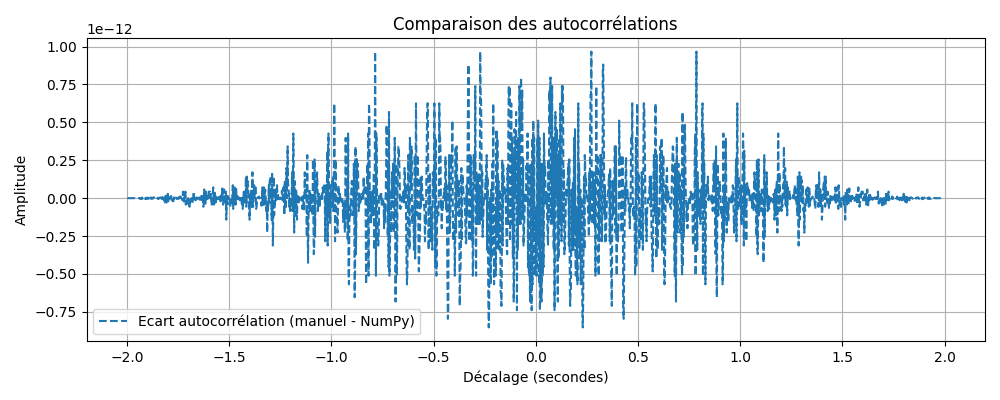
\includegraphics[width=17cm]{screenshots/ecart_autocorrelation.png}
\caption{Ecart entre l'autocorrélation manuelle et celle de numpy}
\end{figure} 

L'ecart est trop petit entre les deux méthodes (de l'ordre de \(10^{-12}\)). Ceci est dû à la précision numérique des calculs et au fait que l'autocorrelation numpy est calculée différemment en utilisant plusieurs techniques d'optimisation.\\

On calcule le rapport des energies entre la différence entre les deux méthodes et l'autocorrelation de numpy :
\[ \text{rapport} = \frac{\sum_{k=0}^{N-1} \text{diff}[k]^2}{\sum_{k=0}^{N-1} \text{autocorr}[k]^2} \]

On trouve plusieurs valeurs de rapport pour différentes valeurs de N. Ceci est dû à la variation de l'énergie du signal en fonction de N, car l'autocorrelation et l'énergie sont sensibles à la longueur du signal (somme de 0 à N-1). On rajoute donc des valeurs au numérateur et au dénominateur dans le calcul de ce rapport (qui ne sont pas équivalentes vu l'écart entre les deux méthodes) ce qui expliques des valeurs de rapport différentes.

\begin{figure}[!h]
\centering
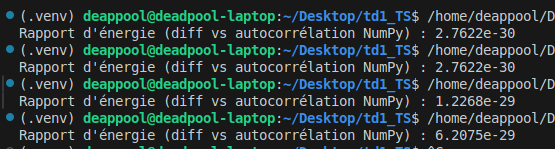
\includegraphics[width=17cm]{screenshots/valeur_rapport.png}
\caption{Valeurs du rapport pour plusieurs valeurs de N}
\end{figure} 